\documentclass[../../../main]{subfiles}


\begin{document}

\section{FreeRTOS}

This section has the purpose of detailing how the software for the Tiva microcontroller is setup and why. The responsibility of the Tiva is to act as the brain of the entire system while the FPGA acts like a data acquisitions device and a hardware controller. 

The operating system used as the platform on the Tiva is FreeRTOS, an open source RealTime operating system created by Real Time Engineers LTD.

FreeRTOS handles system processes of different types by creating "Tasks" that are the run using a preemptive scheduler which allows the system to not only run multiple tasks in "parallel"\footnote{Due to only one core being supported, true parallel is not possible.} but also efficiently allocate the systems resources available.


A task is a single area of responsibility that either by necessity or by convention is combined as a single logical unit. Each task in the system (a full overview can be seen in the task diagram) can then be scheduled based on the priority it has been assigned and whether the task itself has decided that it wants to be scheduled. 

\subsection{Scheduling}

In order to enable the microcontroller to run more then one task some form of scheduling must be implemented. This allows the operating system\footnote{FreeRTOS} to make a choice as to what tasks needs processing capacity at this moment in time. In the FreeRTOS based system running on the Tiva scheduling is done trough a priority based preemption\footnote{The ability to pause and resume processes without the process knowing.} capable implementation.

The preemption capability enables the system to respond quickly to higher priority tasks becoming available for execution rather then waiting for the current task to return on its own potentially taking the CPU forever, it will be paused and the higher priority task executed before the lower priority one is resumed and potentially completed.
 
As mentioned the priority allows the system to select more important\footnote{Defined by the programmer} processes to be run quickly when available.  

The scheduler is run by a timer interrupt every 5ms and during this the current task is paused and the scheduler evaluates the next eligible task to run, this may be the same task that was running before and this will then be resumed, but the scheduler must be run every 5ms tick to ensure correct handling of priorities.

\subsection{Subtask Communication}

The multiple task architecture where each task deals only in their own specific area of the system requires, since the combination of tasks are designed to accomplish one or more high level objective, a way to efficiently communicate between tasks running on the system. 
This is accomplished using a combination of state buffers and queues. 

State buffers are simple buffers keeping the last value written to it until a new value is written regardless of reads performed in that time. The implementation of this concept is done trough variables of the appropriate task being declared in global scope and therefore available to every function in the system.

All queues in the system are FIFO\footnote{First-In-First-Out} queues allowing easy exchange of data between different parts of the system, while maintaining loose coupling between components. This loose coupling allows more parallel development and a more robust end product. 

To maintain data integrity all shared-write resources are protected with semaphores allowing a task to obtain exclusive access to a resource and be able to update it without risk of data corruption caused by interrupted write access.




\subsection{Tasks}

The entire system has been created as a task diagram in figure \ref{fig:entire_task_diagram}. 

There is a number of task that exists only to provide services to other tasks, those tasks are designated system tasks. 

\subsubsection{Status LED task}

This task only exist to toggle an LED on the board to verify that the OS is running and has not encountered some problem that could not be resolved automatically. Therefore the task has been assigned a low priority and will be processed with spare capacity.

\subsubsection{UART Tasks}%

This group consists of the Transmit and Receive task which a created completely independently. The TX task accepts data via a queue and sends that out the system via UART. The RX task is the inverse of this. The tasks are a part of making the system work and therefore run with normal priority. 


\subsubsection{LCD Task}

The LCD task takes items from a queue and adds them to the currently active line on the LCD display. The task is run with low priority as this only need to provide feedback in human observable time frames.

\subsubsection{Matrix Keypad Task}

This task simply adds key presses from the keypad to a queue available to the rest of the system. Is being run with low priority as immediate response is not required for function.

\subsubsection{Serial Peripheral Interface Task}

The SPI task handles all communication between the microcontroller and the FPGA and thus is indirectly responsible for all data acquisition and hardware control. This requires a priority of normal so the task is prioritized but does not require hard timing.  

Besides system tasks there are tasks that can be categorized as being the "application" run on the system. These tasks are designated "user tasks".

\subsubsection{PID}

This group of two tasks handle the control for both axis of the pan-tilt system and are the most critical processes. These run with high priority and therefore the best timing reliability that the system can offer.

\subsubsection{User interface}

% TODO

\begin{figure}[H]
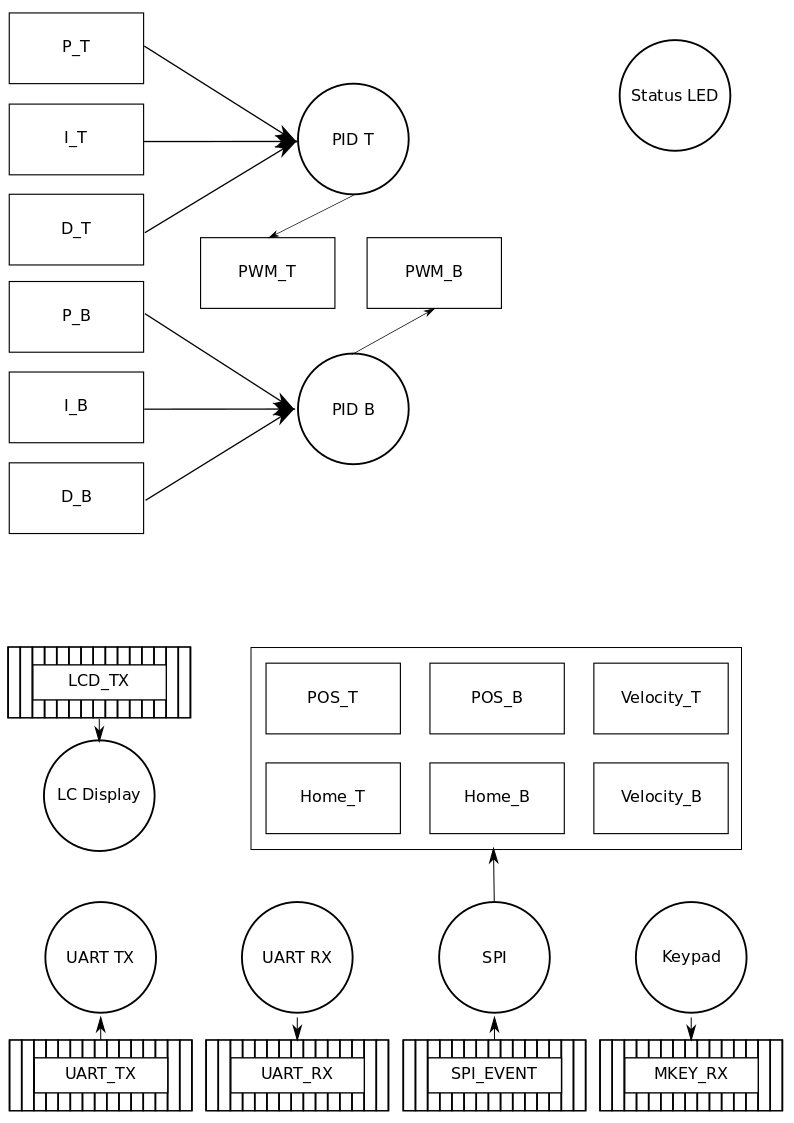
\includegraphics[width=\columnwidth]{taskdiagram_full.png}
\caption{Task Diagram of entire system}
\label{fig:entire_task_diagram}
\end{figure}

\end{document}

